%% This is file `elsarticle-template-1-num.tex',
%%
%% Copyright 2009 Elsevier Ltd
%%
%% This file is part of the 'Elsarticle Bundle'.
%% ---------------------------------------------
%%
%% It may be distributed under the conditions of the LaTeX Project Public
%% License, either version 1.2 of this license or (at your option) any
%% later version.  The latest version of this license is in
%%    http://www.latex-project.org/lppl.txt
%% and version 1.2 or later is part of all distributions of LaTeX
%% version 1999/12/01 or later.
%%
%% Template article for Elsevier's document class `elsarticle'
%% with numbered style bibliographic references
%%
%% $Id: elsarticle-template-1-num.tex 149 2009-10-08 05:01:15Z rishi $
%% $URL: http://lenova.river-valley.com/svn/elsbst/trunk/elsarticle-template-1-num.tex $
%%
\documentclass[preprint,12pt]{elsarticle}

%% Use the option review to obtain double line spacing
%% \documentclass[preprint,review,12pt]{elsarticle}

%% Use the options 1p,twocolumn; 3p; 3p,twocolumn; 5p; or 5p,twocolumn
%% for a journal layout:
%% \documentclass[final,1p,times]{elsarticle}
%% \documentclass[final,1p,times,twocolumn]{elsarticle}
%% \documentclass[final,3p,times]{elsarticle}
%% \documentclass[final,3p,times,twocolumn]{elsarticle}
%% \documentclass[final,5p,times]{elsarticle}
%% \documentclass[final,5p,times,twocolumn]{elsarticle}

%% The graphicx package provides the includegraphics command.
\usepackage{graphicx}
%% The amssymb package provides various useful mathematical symbols
%\usepackage{amssymb}
%% The amsthm package provides extended theorem environments
\usepackage{amsthm}

%% The lineno packages adds line numbers. Start line numbering with
%% \begin{linenumbers}, end it with \end{linenumbers}. Or switch it on
%% for the whole article with \linenumbers after \end{frontmatter}.
\usepackage{lineno}

%% natbib.sty is loaded by default. However, natbib options can be
%% provided with \biboptions{...} command. Following options are
%% valid:

%%   round  -  round parentheses are used (default)
%%   square -  square brackets are used   [option]
%%   curly  -  curly braces are used      {option}
%%   angle  -  angle brackets are used    <option>
%%   semicolon  -  multiple citations separated by semi-colon
%%   colon  - same as semicolon, an earlier confusion
%%   comma  -  separated by comma
%%   numbers-  selects numerical citations
%%   super  -  numerical citations as superscripts
%%   sort   -  sorts multiple citations according to order in ref. list
%%   sort&compress   -  like sort, but also compresses numerical citations
%%   compress - compresses without sorting
%%
%% \biboptions{comma,round}

% \biboptions{}

% \journal{Journal Name}



\usepackage[utf8]{inputenc} % Required for inputting international characters
\usepackage[T1]{fontenc} % Output font encoding for international characters
\usepackage{hyperref}


\newcommand{\propene}{C$_{3}$H$_{8}$}
\newcommand{\ammonia}{NH$_3$}

%Define a command for writing temperature in degree Celsius
\newcommand{\degreeC}[1]{$#1\  ^{\circ}\mathrm{C}$}

%\newcommand{\degreeC}[1]{$#1\, ^{\circ}\mathrm{C}$}


\begin{document}


\begin{frontmatter}

%% Title, authors and addresses

\title{Effect of \propene\ in the kinetic of the adsorption of \ammonia}

%% use the tnoteref command within \title for footnotes;
%% use the tnotetext command for the associated footnote;
%% use the fnref command within \author or \address for footnotes;
%% use the fntext command for the associated footnote;
%% use the corref command within \author for corresponding author footnotes;
%% use the cortext command for the associated footnote;
%% use the ead command for the email address,
%% and the form \ead[url] for the home page:
%%
%% \title{Title\tnoteref{label1}}
%% \tnotetext[label1]{}
%% \author{Name\corref{cor1}\fnref{label2}}
%% \ead{email address}
%% \ead[url]{home page}
%% \fntext[label2]{}
%% \cortext[cor1]{}
%% \address{Address\fnref{label3}}
%% \fntext[label3]{}


%% use optional labels to link authors explicitly to addresses:
%% \author[label1,label2]{<author name>}
%% \address[label1]{<address>}
%% \address[label2]{<address>}

\author{Andrés Camilo Álvarez Montoya}

\address{Freiberg, Germany}

\begin{abstract}
%% Text of abstract
In this report I will show the results I Obtained in my internship in the institute of energy process engineering and chemical engineering.
\end{abstract}

\begin{keyword}
Cu-SAPO-34 \sep Cu-ZSM-5 \sep \propene \sep \ammonia\ desorption kinetic.
%% keywords here, in the form: keyword \sep keyword

%% MSC codes here, in the form: \MSC code \sep code
%% or \MSC[2008] code \sep code (2000 is the default)

\end{keyword}

\end{frontmatter}

%%
%% Start line numbering here if you want
%%
\linenumbers

%% main text
\section{Experimental}
\label{S:1}

\subsection{Catalysts synthesis}
SAPO-34 was synthesized according to the hydrothermal method. Aluminum, phosphorous, and silicon sources were, aluminum isopropoxide, orthophosporic acid, and tetraethyl ortosilicate respectively. The structural directing agent was morpholine and the solvent was water. All the compounds were mixed together in a Al$_2$O$_3$:P$_2$O5:SiO$_2$:SDA:H$_2$O molar ratio of 1:1:0.6:4:70. Aluminum isopropoxide and morpholine was added to the water and stirred for 15 min. Then TEOS was added to the solution under stirring for another 15 min. Finally, the H$_3$PO$_4$ was added dropwise and let the stirring for 1 h. The solution was transferred to TEFLON autoclaves and the crystallization was made at \degreeC{200} for 14 hours. The final solution was dried at \degreeC{120} for 12 h and calcined at \degreeC{560} for 12 h. The copper incorporation was made by the ion exchange method according to the procedure use by Olsson et al. SAPO-34 was submitted at ion exchange with a solution NH$_4$NO$_3$ 5.4 M in a ration of 7 mL of solution per gram of SAPO-34 1 h at \degreeC{80} maintaining the pH between 3.0 $-$ 3.5. The solid was dried at \degreeC{120} overnight and the ion exchange was repeated. Finally, the solid was calcined at \degreeC{560} for 12 h for obtaining the H-SAPO-34 form. The H-SAPO-34 was ion exchanged with $\mathrm{CuNO_3\cdot2.5H_2O}$

NH$_4$-ZSM-5 CBV2340E was purchased from Zeolyst International. The sample was calcined at \degreeC{560} for 5 h for obtaining the H-ZSM-5 form. The H-ZSM-5 sample was ion exchanged with Cu(CH$_3$COO)$_2$ containing 160 ppm Cu 125 mL of solution per gram of zeolite. The solution was filtered with destilled water, dried at \degreeC{120} for 12 h and calcined in synthetic air for 5 h at \degreeC{560}.

%\begin{itemize}
%\item Bullet point one
%\item Bullet point two
%\end{itemize}

%\begin{enumerate}
%\item Numbered list item one
%\item Numbered list item two
%\end{enumerate}

%\begin{table}[h]
%\centering
%\begin{tabular}{l l l}
%\hline
%\textbf{Treatments} & \textbf{Response 1} & \textbf{Response 2}\\
%\hline
%Treatment 1 & 0.0003262 & 0.562 \\
%Treatment 2 & 0.0015681 & 0.910 \\
%Treatment 3 & 0.0009271 & 0.296 \\
%\hline
%\end{tabular}
%\caption{Table caption}
%\end{table}


\subsection{Catalyst characterization}
XRD

Area BET was determined in a Micromeritics ASAP 2020 equipment. The sample was pretrated at \degreeC{350} for 2 h and the isotherm was recorded at -\degreeC{196}.

Diffuse reflectance UV-Vis spectra were recorded on a Lambda 850 Perkin Elmer spectrometer equipped with a Praying mantis reflectance optics (Harrick Scientific). The measurements were performed under ambient conditions between 200 and 800 nm with a resolution of 0.9 nm. Data were obtained in \%R and then transformed into Kubelka-Munk function using Eq. (\ref{eq:Kubelka}), in which R is the ratio of the reflectance of the Cu-exchanged sample and bare sample.

SEM-EDS were performed on a FEI Quanta FEG 250 scanning electron microscope

Cu content ICP

IR


\begin{equation}
F(R) = 1 - \frac{R^2}{2R}
\label{eq:Kubelka}
\end{equation}


\subsection{\ammonia\ adsorption/desorption experiments}
Figure \ref{fig:NH3-TPD system} shows the bench reactor for performing the \ammonia-TPD experiments. Typically, 200 mg of granulated (120 - 250 $\mu$m) catalyst was packed into a quartz reactor (i.d. 8mm). The sample was placed in between quartz wool and the temperatures were measure just in front and behind the the bed. Flows were controlled by Bronkhorst mass flow controllers. Before the experiments the sample was pretreated with synthetic air at \degreeC{450} at a flowrate of 500 mL/min. Then, it was let to cool down to the adsorption temperature in 500 mL/min of N$_2$. The saturation was perfomed with 1000 ppm \ammonia\ in nitrogen until complete saturation at a flow of 500 mL/min. Then, a flusing with 500 mL/min N$_2$ was made in order to remove physisorbed \ammonia. The desorption was carry out at a heating rate of \degreeC{10}/min from adsorption temperature until \degreeC{600}. Concentration of \ammonia\ was measure via nondispersive infrared (NDIR) spectrometer (DINOS 1.b from Leybold-Heraeus).

The NH$_X$ species on the surface of the catalysts was determined by in situ DRIFTS spectroscopy. A Tensor 27 FTIR spectrometer (Bruker) equipped with a liquid-nitrogen cooled MCT detector. A Praying Mantis reflectance optics (Harrick Scientific) heatable stainless steel infrared cell with ZnSe windows was used. The cell was connected to a gas-handling system. In a typical experiment, 30 mg of sample was put into the cup of the cell and treated at \degreeC{450} in 500 mL/min N$_2$ for 20 min. Then, it was cooled to the adsorption temperatures and the background spectra were taken in N$_2$ flow from \degreeC{200} until \degreeC{50} in \degreeC{50} steps. At this temperature, the flow of 1000 ppm \ammonia\ was introduced for 30 min and then flushed for 1 h. Then the DRIFTS spectra were taken from \degreeC{50} until \degreeC{200} in \degreeC{50} steps. All DRIFTS spectra were collected in the range of 4000$-$650 cm$^{-1}$ by accumulating 600 scans at a 4 cm$^{-1}$ resolution. The analysis of the data was made via the Kubelka-Munk function.


\begin{figure}
\centering
\centering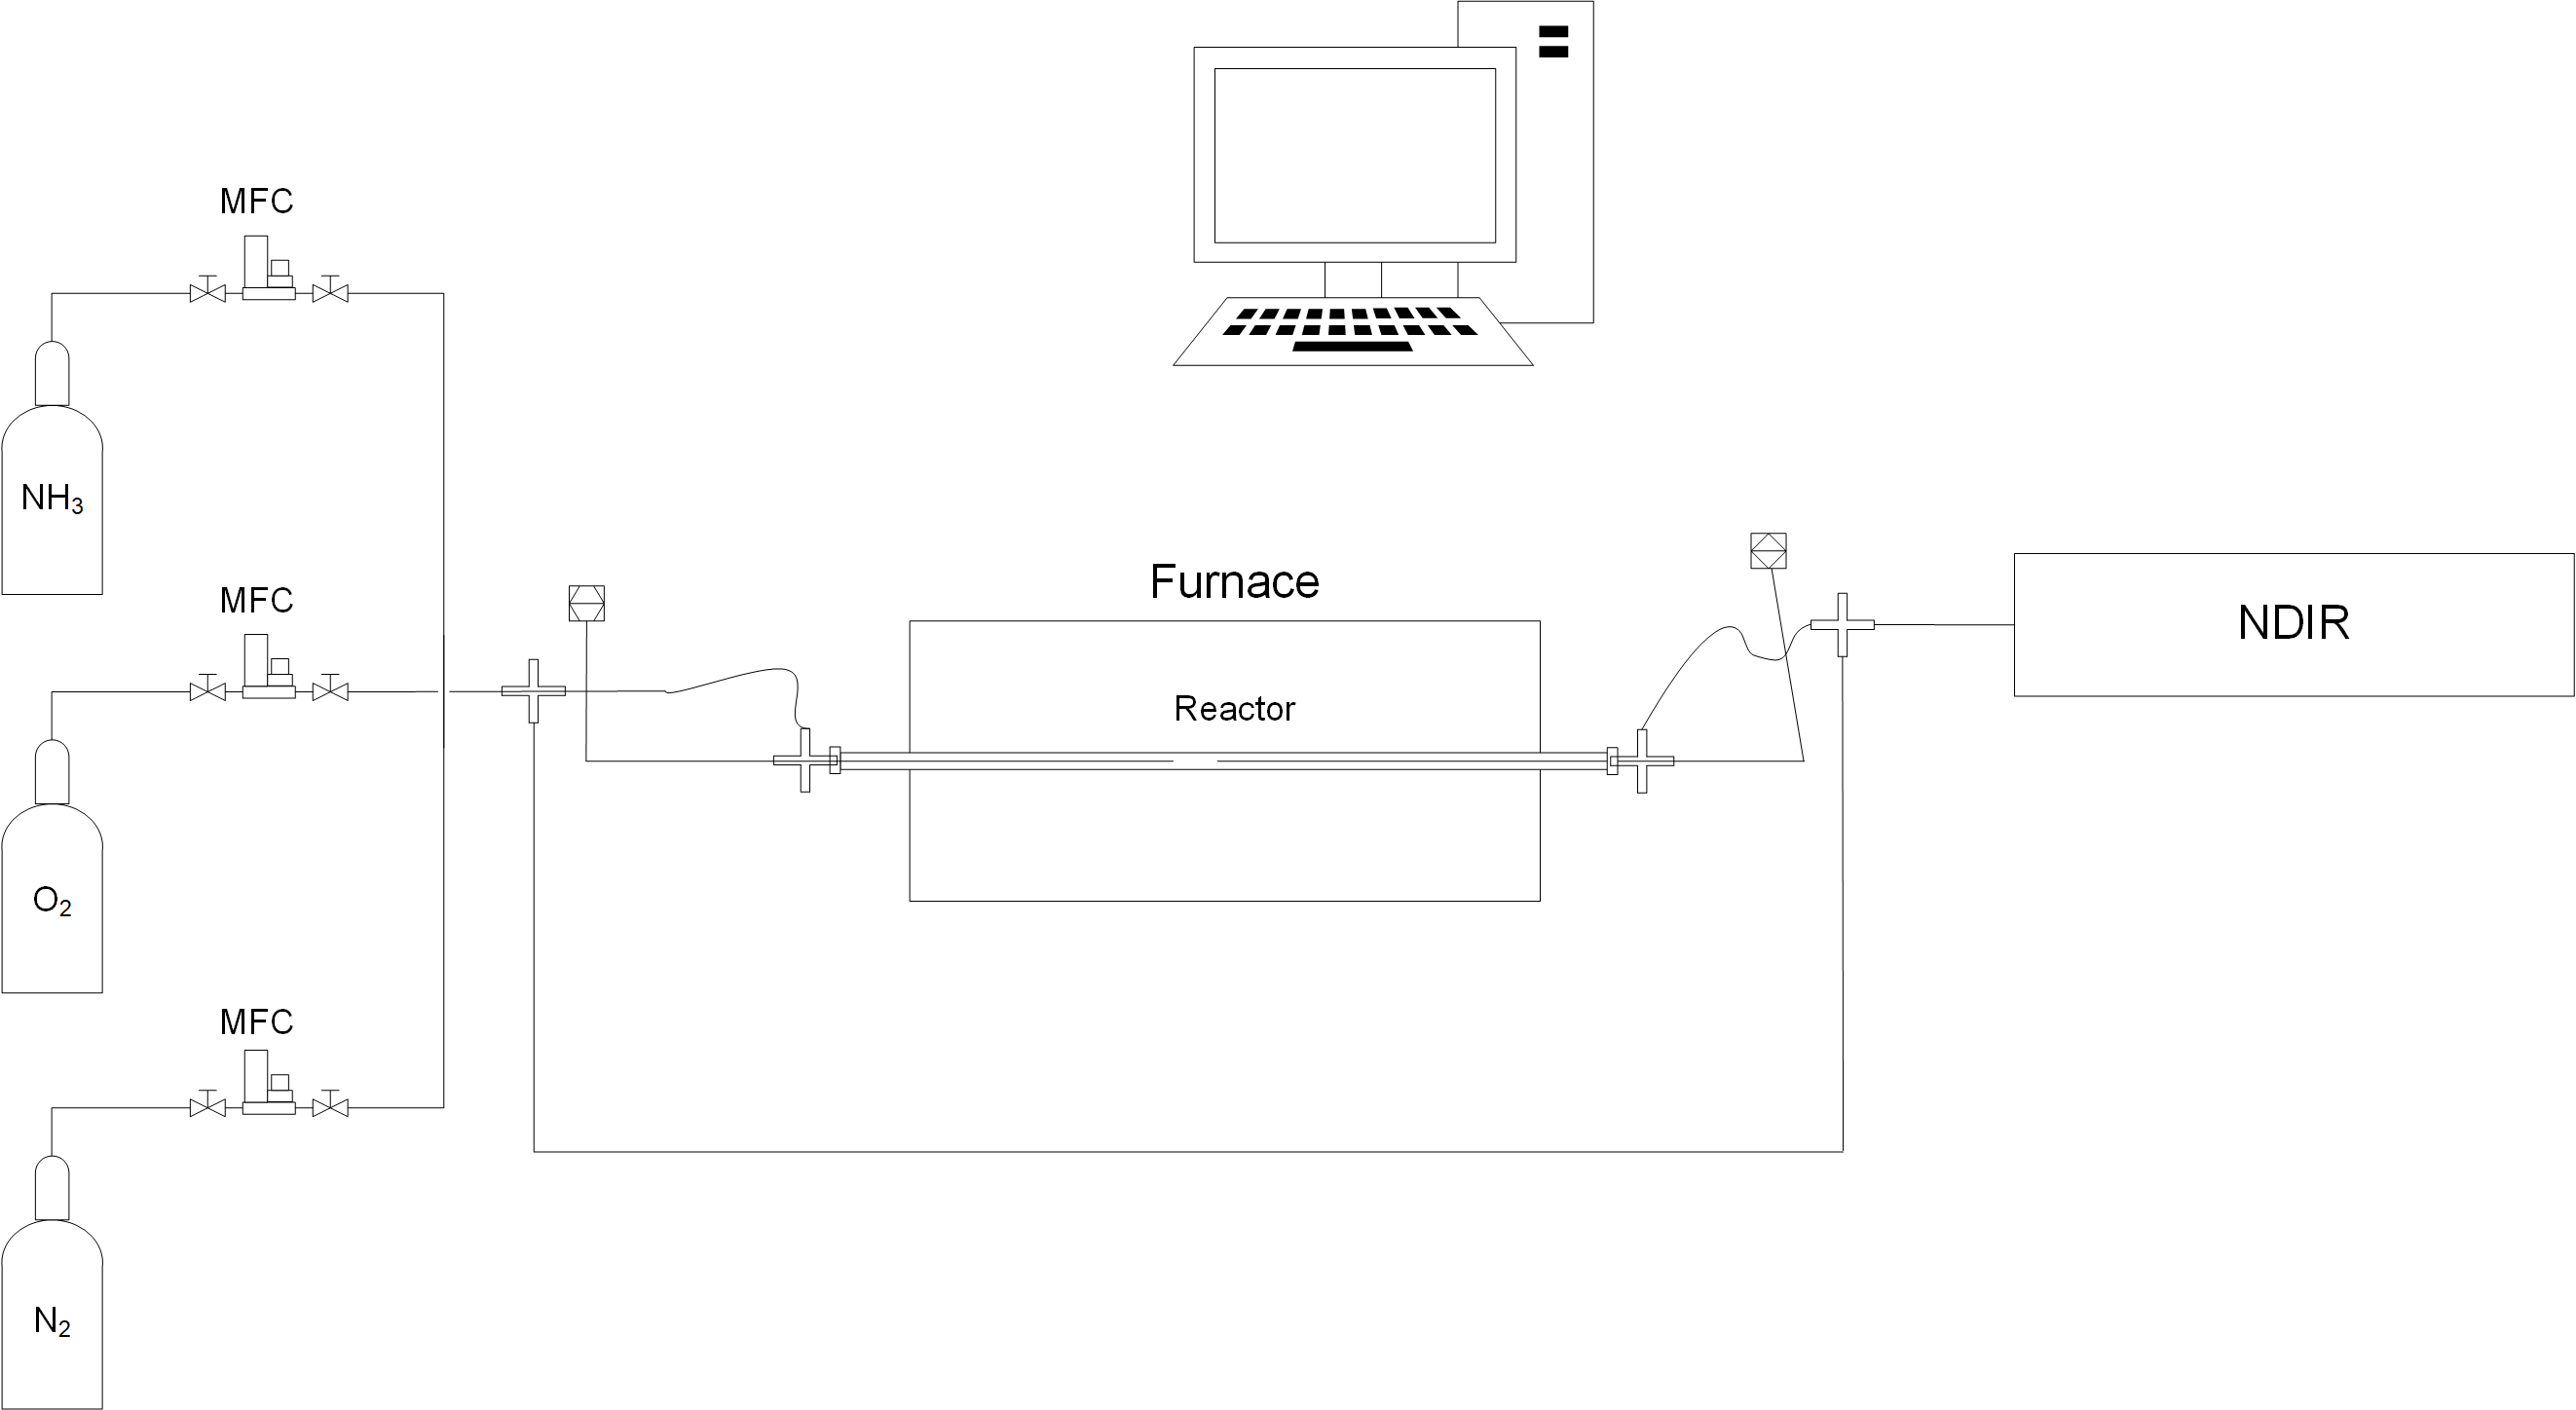
\includegraphics[width=0.95\linewidth]{Figures/NH3TPD_fig.png}
\caption{\ammonia-TPD system for experiments}
\label{fig:NH3-TPD system}
\end{figure}


\section{Results}
\label{S:2}

\subsection{Catalyst characterization}

Figure \ref{fig:DRUV-Vis Cu-SAPO-34} shows the DRUV-Vis spectra of the Cu-SAPO-34 sample. Two characteristic bands can be seen, the fist one at about 200 nm was attributed to a charge transfer from O to Cu$^{+}$/Cu$^{2+}$ and the band at around 750 nm to d-d transition of isolated Cu$^{2+}$ \cite{Leistner2017ImpactCu/SAPO-34}. Area BET of the bare sample was 550 m$^2$/g and for the ion-exchanged with Cu was 301 m$^2$/g.

\subsection{\ammonia-TPD}



\begin{figure}
    \centering
    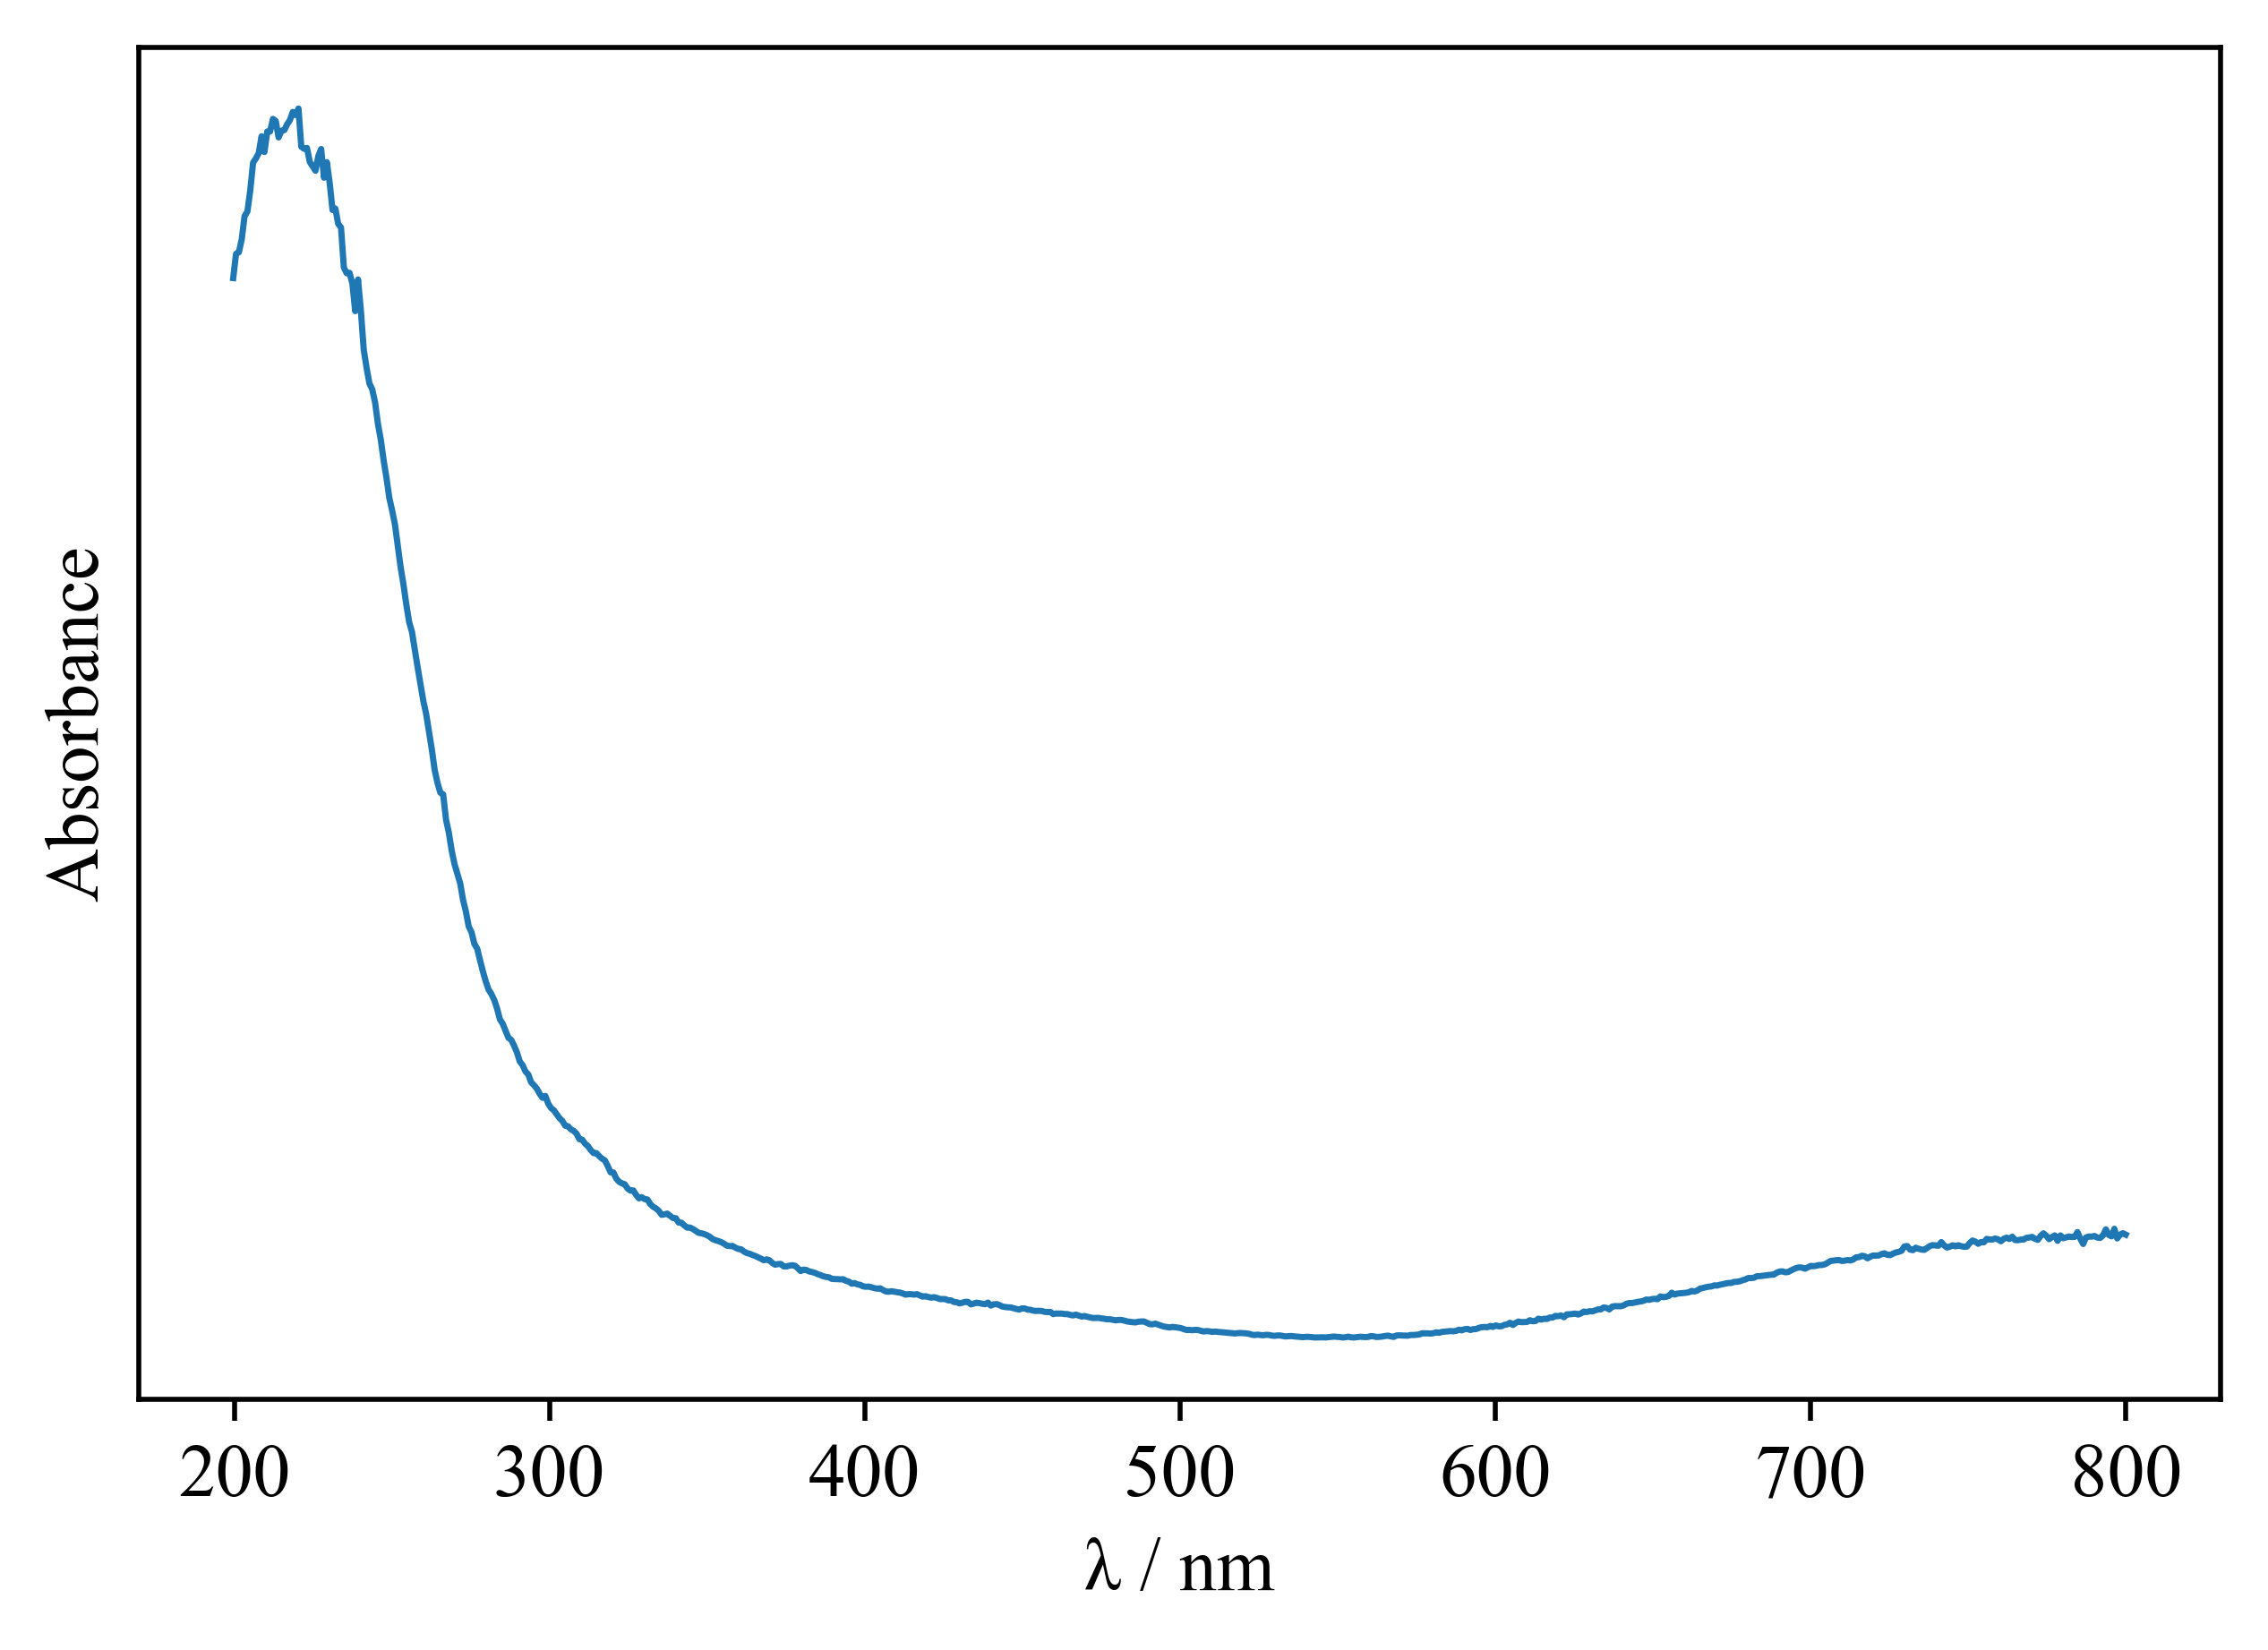
\includegraphics[width=0.95\linewidth]{Figures/Cu_SAPO_34_absorbance.png}
    \caption{DRUV-Vis spectra of Cu-SAPO-34}
    \label{fig:DRUV-Vis Cu-SAPO-34}
\end{figure}


\begin{figure}
    \centering
    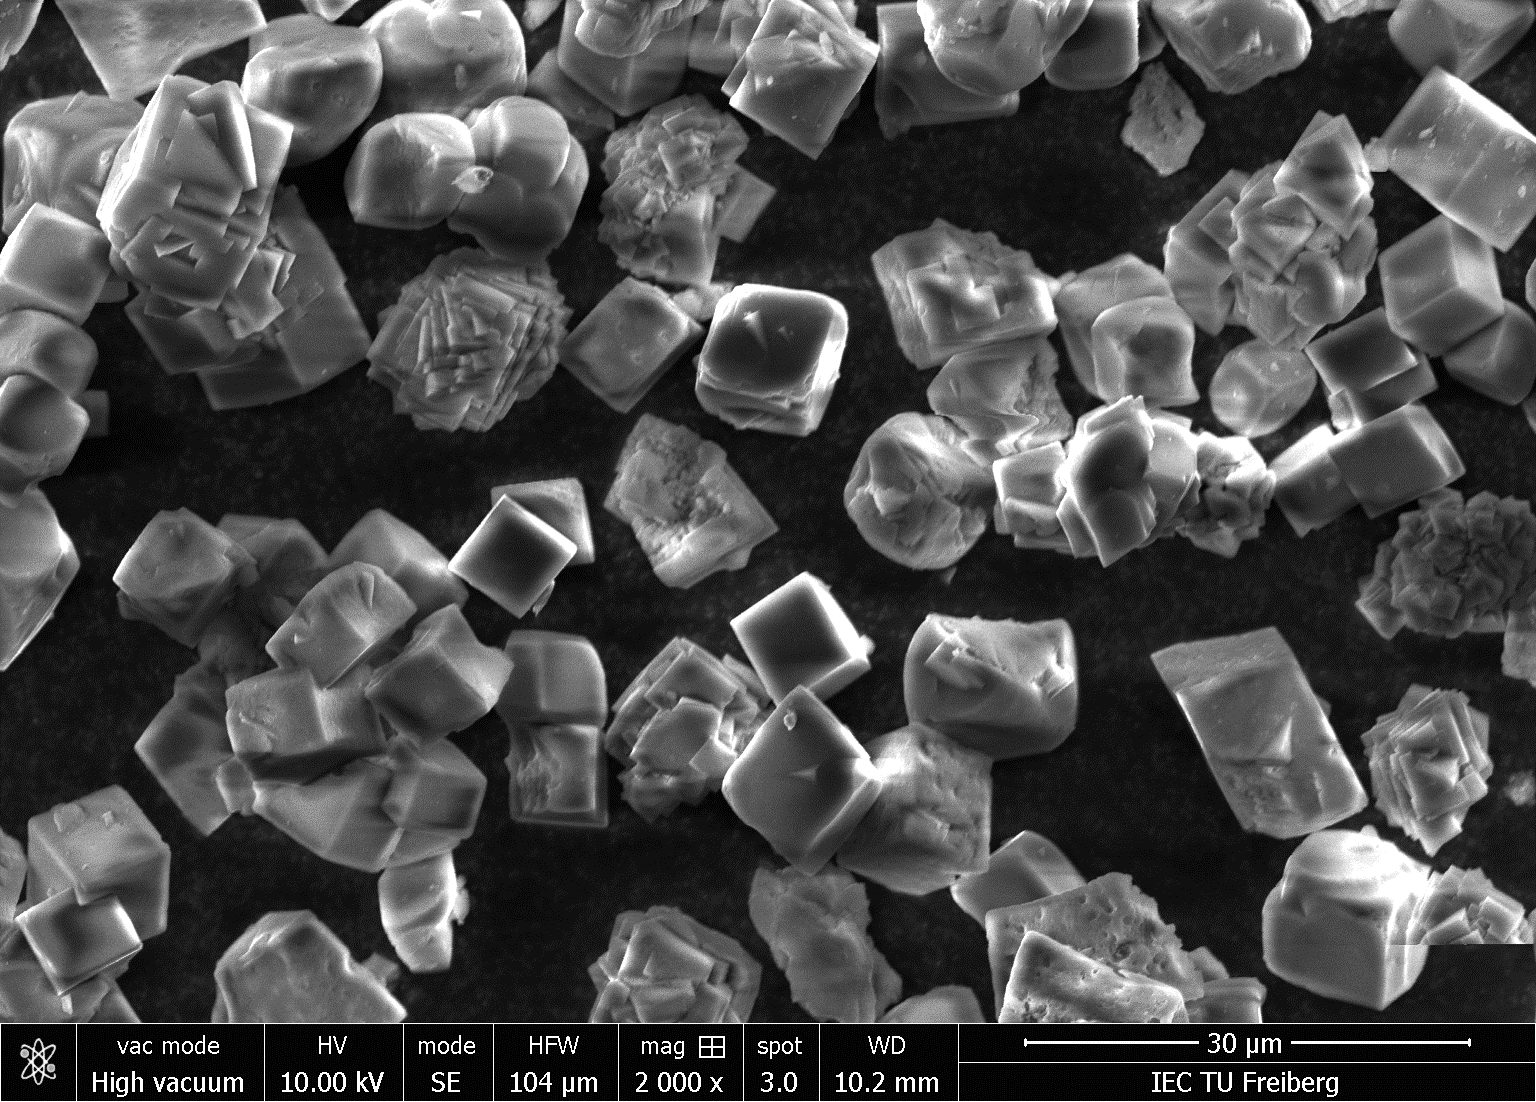
\includegraphics[width=0.95\linewidth]{Figures/SEM-Cu-SAPO-34.png}
    \caption{SEM micrograph of Cu-SAPO-34}
    \label{fig:SEM Cu-SAPO-34}
\end{figure}


%% The Appendices part is started with the command \appendix;
%% appendix sections are then done as normal sections
%% \appendix

%% \section{}
%% \label{}

%% References
%%
%% Following citation commands can be used in the body text:
%% Usage of \cite is as follows:
%%   \cite{key}          ==>>  [#]
%%   \cite[chap. 2]{key} ==>>  [#, chap. 2]
%%   \citet{key}         ==>>  Author [#]

%% References with bibTeX database:

\bibliographystyle{model1-num-names}
\bibliography{references.bib}

%% Authors are advised to submit their bibtex database files. They are
%% requested to list a bibtex style file in the manuscript if they do
%% not want to use model1-num-names.bst.

%% References without bibTeX database:

% \begin{thebibliography}{00}

%% \bibitem must have the following form:
%%   \bibitem{key}...
%%

% \bibitem{}

% \end{thebibliography}


\end{document}

%%
%% End of file 'elsarticle-template-1-num.tex'.